\documentclass[11pt]{article}
\usepackage[utf8]{inputenc}\usepackage[T1]{fontenc}
\usepackage[margin=20mm]{geometry}\usepackage{tikz}\usetikzlibrary{arrows.meta,positioning}
\usepackage{hyperref}\usepackage{longtable}
\begin{document}
\section*{Declarative room structure (P1a)}
Created-at: 2026-09-27 02:45 +02:00. Authorization 2026-09-27 (after 02:13): P1a now, inherited-field
resolution in \texttt{hymeko\_query}; (after 02:20): commit the uncommitted Transformation and SDK state
first as separate prior commits (done: \texttt{transformation} dc002b2, \texttt{hymeko\_web}
da94b0b, both on \texttt{feat/declarative-room}). Standing rule: commit and push, new feat branch
per repository. Predicates, declared conditions and HySTL stay with the RL line.

\paragraph{ETA} WP1 1--1.5 h (until about 04:15). WP2--WP4 3--5 h after the vocabulary decision
below. Basis: WP1 is one extracted reader, one delegation and focused tests; WP2 is a projection
of the size of \texttt{SpatialQuery} plus two model sources and equivalence tests.

\paragraph{Findings that shape the plan}
\begin{enumerate}
\item The own-then-bases field reader exists once, crate-private:
  \texttt{hymeko\_geometry::kinematics::actuation::Fields::child} (own declaration first, then
  bases in authored order, cycle-safe). \texttt{hymeko\_webxr}'s \texttt{attr\_value},
  \texttt{hymeko\_query}'s \texttt{MatchContext::get\_field} and the SDK inspector read direct
  children only; inheritance tests exist in three places (\texttt{decl\_inherits},
  \texttt{isa\_transitive}, \texttt{check\_inherits\_simple}).
\item Two marker vocabularies coexist: ROS (\texttt{ros.marker}: \texttt{dictionary},
  \texttt{marker\_id}, \texttt{size\_m}; \texttt{ros.registration}) used by the deployed room, and
  the spatial one (\texttt{spatial.kinds.fiducial\_anchor}: \texttt{family}, \texttt{identifier},
  \texttt{size\_m}; \texttt{@fiducial\_registration}) with a type-bound query
  (\texttt{hymeko\_webxr::SpatialQuery}).
\item The ecosystem map lists \texttt{hymeko\_webxr} as used by \texttt{hymeko\_quest}; no XR, SDK,
  Kawamirai or HIVE source uses it (finding: map and code disagree).
\item \texttt{hymeko\_query}'s integration target includes \texttt{bench\_workflow}, an un-ignored
  timing \texttt{\#[test]} (finding; not changed by this plan).
\end{enumerate}

\begin{center}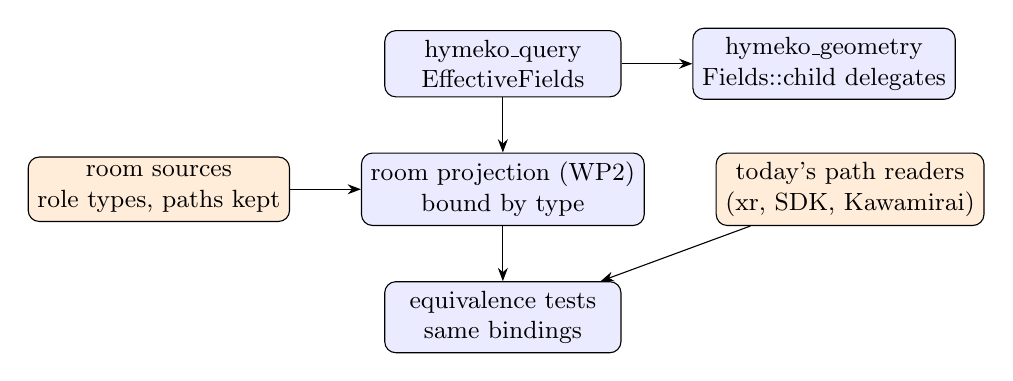
\begin{tikzpicture}[>=Stealth,font=\small,node distance=7mm and 9mm,
  box/.style={draw,rounded corners,align=center,minimum width=30mm,fill=blue!8},
  ext/.style={draw,rounded corners,align=center,minimum width=30mm,fill=orange!15}]
\node[box] (fields) {hymeko\_query\\EffectiveFields};
\node[box,right=of fields] (geom) {hymeko\_geometry\\Fields::child delegates};
\node[box,below=of fields] (room) {room projection (WP2)\\bound by type};
\node[ext,left=of room] (src) {room sources\\role types, paths kept};
\node[ext,right=of room] (old) {today's path readers\\(xr, SDK, Kawamirai)};
\node[box,below=of room] (eq) {equivalence tests\\same bindings};
\draw[->] (fields)--(geom); \draw[->] (fields)--(room); \draw[->] (src)--(room);
\draw[->] (room)--(eq); \draw[->] (old)--(eq);
\end{tikzpicture}
\end{center}

\paragraph{Work packages}
\begin{longtable}{p{10mm}p{150mm}}
WP1&\texttt{hymeko\_query}: public effective-field reader (own declaration, then bases in
authored order, cycle-safe, bounded), with a dotted-path form on \texttt{MatchContext} that is
opt-in (the existing \texttt{get\_field} keeps its direct-child semantics, so template emitters
do not change output). \texttt{hymeko\_geometry::Fields::child} delegates to it.\\
WP2&Room projection (\emph{decision pending}): typed views of room root marker, landmarks,
tracked headset, robot marker and editable room objects, bound by type through queries, never by
path. Option A: extend \texttt{hymeko\_webxr} (spatial owner per ecosystem map and AGENTS.md) and
align the ROS marker with \texttt{fiducial\_anchor}. Option B: room vocabulary beside the ROS one,
projection in the SDK next to \texttt{RoomLayout}.\\
WP3&Model sources: role types on the deployed room (paths unchanged) and a typed rewrite of
\texttt{hive-room.hymeko}; CLI gate for each file.\\
WP4&Equivalence tests: for both sources, today's path-based readers and the new projection yield
the same bindings; README, symbols, duplication, report; commits and push per repository.\\
\end{longtable}

\paragraph{Affected files (WP1)} \texttt{hymeko\_query/src/\{lib.rs, fields.rs (new), rewrite/match\_context.rs\}},
\texttt{hymeko\_geometry/src/kinematics/actuation.rs}, tests in both crates, \texttt{SYMBOLS.md}.
WP2--WP4 files are listed in the amendment after the decision.
\textbf{CORE.YAML items touched:} none (Transformation declares none; Core is not edited).

\paragraph{Interface changes (WP1)} New \texttt{hymeko\_query::EffectiveFields} (child, value);
\texttt{MatchContext::effective\_field(path)}. No existing signature changes.

\paragraph{Amendment 2026-09-27 02:47 +02:00} A separate \texttt{EffectiveFields} struct repeated
\texttt{QueryEngine}'s \texttt{ir}/\texttt{resolver} holder (token clone, +2/+16 against dc002b2).
The reader is therefore \texttt{QueryEngine::effective\_child(decl, key)} and
\texttt{effective\_value(decl, key)} (module \texttt{fields.rs}); \texttt{QueryEngine::ir()} and
\texttt{resolver()} now return the engine's \texttt{'a} borrow, so a value outlives a temporary
engine (widening, source-compatible for callers). Duplication back to 384 clones / 6053 lines.

\paragraph{Amendment 2026-09-27 03:11 +02:00 (WP2--WP4, user decisions after 02:51)} Option A: the
room builds on the spatial vocabulary in \texttt{hymeko\_webxr}. Approved dependencies:
\texttt{hymeko\_webxr} $\rightarrow$ \texttt{hymeko\_query}; \texttt{hymeko\_quest} $\rightarrow$
\texttt{hymeko\_webxr}; generated, byte-checked vocabulary copies beside the room sources.
ETA 3.5--4 h (until about 07:00).
\begin{itemize}
\item \textbf{WP2} (\texttt{transformation}): new \texttt{data/webxr/meta\_room.hymeko} importing
  \texttt{meta\_spatial}: kinds \texttt{room} (scene), \texttt{room\_frame} (spatial frame),
  \texttt{aruco\_marker} (fiducial anchor with defaults \texttt{fiducial\_kind "aruco"},
  \texttt{convention}), \texttt{tracked\_device} (spatial frame). No observation slot on a kind:
  a slot inherited from a kind would be shared by every instance. The root is expressed as a
  relation, reusing \texttt{@fiducial\_registration (+ room\_frame, \textasciitilde{} marker)}.
  New \texttt{RoomQuery} (\texttt{src/room.rs}): rooms, the room frame (exactly one), the optional
  root registration (at most one), landmarks (other fiducials inside the room), tracked devices,
  and all ArUco markers of the model, each with its own \texttt{sample} slot; fields read through
  \texttt{QueryEngine::effective\_value}. \texttt{SpatialQuery}'s attribute reads use the same
  effective rule (a kind's default is inherited; the validator's reserved-field check stays
  direct). Vocabulary texts exported as constants for the copy check.
\item \textbf{WP3} (\texttt{middleware\_hymeko}, new \texttt{feat/declarative-room}): copies of
  \texttt{meta\_spatial.hymeko} and \texttt{meta\_room.hymeko} in \texttt{examples/}, written by
  \texttt{hymeko\_webxr/tools/sync-vocabulary.ps1}; \texttt{ros-ur5.hymeko} imports them; the room
  becomes \texttt{+ <isa> room} with a room frame and the root registration; the five markers and
  the headset gain the spatial bases; markers gain \texttt{family}/\texttt{identifier} beside
  \texttt{dictionary}/\texttt{marker\_id} (expand step; readers switch in P2). Paths unchanged;
  \texttt{ros.meta.hymeko} unchanged (two middleware tests compile it standalone and imports are
  not transitive). \texttt{hive-room.hymeko} unchanged: it declares no marker or device.
  Room objects stay with \texttt{RoomLayout} (the kit is appended to arbitrary workspaces and
  cannot import the vocabulary); typing them is a P2 item.
\item \textbf{WP4} (\texttt{xr}, new \texttt{feat/declarative-room}): \texttt{hymeko\_quest} test
  dependency use of \texttt{RoomQuery}: for the UR5 room and \texttt{hive-room}, the path readers
  in \texttt{lan.rs} (\texttt{marker\_at}, landmarks, observer slot) and \texttt{RoomQuery} yield the
  same root, landmark set and headset slot; \texttt{family}/\texttt{identifier} equal
  \texttt{dictionary}/\texttt{marker\_id}; the middleware copies equal the exported vocabulary.
  CLI gate on \texttt{meta\_room.hymeko} and \texttt{ros-ur5.hymeko}; middleware tests re-run.
\end{itemize}
Affected files: \texttt{transformation/hymeko\_webxr/\{Cargo.toml, src/lib.rs, src/query.rs,
src/room.rs, data/webxr/meta\_room.hymeko, tools/sync-vocabulary.ps1, tests\}},
\texttt{Cargo.lock}; \texttt{middleware\_hymeko/examples/\{ros-ur5.hymeko, meta\_spatial.hymeko,
meta\_room.hymeko\}}, README; \texttt{xr/hymeko\_quest/\{Cargo.toml, src/lan.rs\}}, \texttt{Cargo.lock}, README.
CORE.YAML items touched: none.

\paragraph{Tests} Unit: own value overrides a base; bases in authored order; multi-level
inheritance; diamond and cycle terminate; missing field; dotted path through an inherited block.
Regression: \texttt{hymeko\_geometry} inherited-material/geometry and actuation tests unchanged.
Correctness only; \texttt{-{}-skip bench\_} for the query integration target; no measurement.

\paragraph{Budgets} Reader cost is bounded by the base graph (visited set); no allocation per
direct hit beyond the walk stack. No performance measurement is authorized.

\paragraph{Rollback} Revert the WP1 commit; geometry returns to its private reader.

\paragraph{Risks} (1) Changing \texttt{get\_field} globally would change emitted URDF/SDF; the new
reader is opt-in. (2) The vocabulary decision changes a deployed model (WP3); live HIVE room
migration is P2 and not part of this plan. (3) Dirty sibling state is now committed but still
depends on uncommitted Core APIs; builds are local integration builds.
\end{document}
